%%%%%%%%%%%%%%%%%%%%%%%%%%%%%%%%%%%%%%%%%
% Jacobs Landscape Poster
% LaTeX Template
% Version 1.0 (29/03/13)

% This template has been downloaded from:
% http://www.LaTeXTemplates.com
%
%%%%%%%%%%%%%%%%%%%%%%%%%%%%%%%%%%%%%%%%%
% Esta plantilla corresponde al formato de póster para el Simposio Internacional de Estadística. Este póster esta predeterminado para español y dos columnas. Tanto en el póster como en los comentarios encontrará una guía para su desarrollo. Si usted desea agregar el logosímbolo de su institución, este se encuentra en beamerthemeconfposter.sty

%----------------------------------------------------------------------------------------
%	PAQUETES Y OTRAS CONFIGURACIONES DEL DOCUMENTO
%----------------------------------------------------------------------------------------

\documentclass[final]{beamer}

\usepackage[scale=1.24]{beamerposter2} % Paquete beamerposter para crear el poster
\usepackage{graphicx}
\usepackage{array}
\usepackage{tabu}
\usepackage{multicol}
\usepackage{multirow}
\usepackage{anyfontsize}

\usetheme{confposter} % Utilice el tema confposter suministrado con esta plantilla

\setbeamercolor{block title}{fg=ngreen,bg=white} % Colores del título de bloque 
\setbeamercolor{block body}{fg=black,bg=white} % Colores del cuerpo de bloque 
\setbeamercolor{block alerted title}{fg=white,bg=dgreen!70} % Colores del título de bloque resaltado 
\setbeamercolor{block alerted body}{fg=black,bg=dblue!10} % Colores del cuerpo de bloque resaltado
% Muchos más colores están disponibles para su uso en beamerthemeconfposter.sty

%-----------------------------------------------------------
% Defina los anchos de las columnas y el tamaño total del cartel
% Configure valores efectivos de ancho de separación de columna (sepwid), ancho de primera columna (onecolwid) y ancho de segunda columna (twocolwid), primero elija cuántas columnas quiere y cuánta separación quiere entre columnas
% En esta plantilla , el ancho de separación elegida es 0.024 del ancho del poster y dispuesta para tres columnas

% Por tanto, onecolwid debe ser (1-(# de columnas+1)*sepwid)/# de columnas e.g. Si se disponen cuatro columnas, entonces (1-(4+1)*0.024)/4 = 0.22
% Para nuestro caso (1-(3+1)*0.024)/3 = 0.3013
% Se define twocolwid como: (2*onecolwid)+sepwid = 0.464
% Se define threecolwid como: (3*onecolwid)+2*sepwid = 0.708



\newlength{\sepwid}
\newlength{\onecolwid}
\newlength{\twocolwid}
\newlength{\threecolwid}
\setlength{\paperwidth}{39.3in} % ancho A0: 48in
\setlength{\paperheight}{59in} % alto A0: 36in
\setlength{\sepwid}{0.03\paperwidth} % Ancho de separación (espacio blanco) entre columnas
\setlength{\onecolwid}{0.45\paperwidth} % 0.22 Ancho de una columna
\setlength{\twocolwid}{0.45\paperwidth} % 0.464 Ancho de dos columnas
%\setlength{\threecolwid}{0.9519\paperwidth} % 0.708 Ancho de tres columnas
\setlength{\topmargin}{-0.in} % Reduce la medida del margen superior
%-----------------------------------------------------------

\usepackage{graphicx}  % Se requiere para incluir imagenes

\usepackage{booktabs} % Reglas superior e inferior para las tablas

\def\figurename{Figura}
\def\tablename{Tabla}
%----------------------------------------------------------------------------------------
%	SECCIÓN DEL TÍTULO
%----------------------------------------------------------------------------------------
\title{Formato de Poster para Simposio de Estadística de la Universidad Nacional de Colombia} % Título del poster

\author{{\Large Autor(es)}} % Autor(es)

\institute{{\Large Institución(es)}} % Institución(es)
%----------------------------------------------------------------------------------------
% INICIO DEL DOCUMENTO
\begin{document}    

\addtobeamertemplate{block end}{}{\vspace*{1ex}} % Espacio en blanco bajo los bloques
\addtobeamertemplate{block alerted end}{}{\vspace*{1ex}} % espacio en blanco bajo los bloques resaltados

\setlength{\belowcaptionskip}{1ex} % Espacio en blanco bajo las imagenes
\setlength\belowdisplayshortskip{1ex} % Espacio en blanco bajo las ecuaciones

\begin{frame}[t] % Todo el poster esta en el entorno one beamer frame

\begin{columns}[t] % El cartel completo consta de dos columnas principales

\begin{column}{\sepwid}\end{column} 

\begin{column}{\onecolwid} % Inicio de la Primera columna

%----------------------------------------------------------------------------------------
%	RESUMEN
%----------------------------------------------------------------------------------------

\begin{alertblock}{Resumen}
	Coloque aquí un resumen de máximo 550 caracteres incluyendo espacios, o 80 palabras. \textbf{Ejemplo:} Para lograr este cometido haga uso de dos metodologías de la Investigación de Operaciones: Programación Dinámica y Simulación. La programación dinámica permite determinar la distribución del recurso para cada uno de los canales de venta; y al agregarle algunos conceptos (valor esperado y robustez), podemos determinar diferentes escenarios, obteniendo así los propuestos: Indiferencia al riesgo, Amante al riesgo, y Adverso al riesgo. Por su parte con la simulación, se ha modelado el comportamiento del funcionamiento de un hotel básico.
\end{alertblock}

%----------------------------------------------------------------------------------------
%	OBJETIVOS
%----------------------------------------------------------------------------------------

\begin{block}{Objetivos}
Incluya máximo 3 objetivos: el objetivo general y un par de objetivos específicos como se muestra a continuación.
\begin{itemize}
    \item Ejecutar la programación dinámica y simulación en el contexto de esta investigación.
    \item Determinar la distribución del recurso para cada uno de los canales de venta.
    \item Modelar el comportamiento del funcionamiento de un hotel básico.
\end{itemize}    

\end{block}

\begin{block}{Metodología}
Numere en máximo 4 pasos el desarrollo del trabajo:
	\begin{itemize}
	\item Obtención y depuración los datos.
    \item Creación de los algoritmos de programación dinámica y simulación.
    \item Verificación de las distribuciones resultantes de la simulación realizada.
	\item Análisis de los resultados obtenidos.
	\end{itemize}
\end{block}
%------------------------------------------------

%----------------------------------------------------------------------------------------
%	RESULTADOS Y ANÁLISIS
%----------------------------------------------------------------------------------------

\begin{block}{Resultados y análisis}
Esta columna está completamente destinada para los resultados y análisis de su investigación / trabajo. Puede agregar gráficos, tablas y los resultados que considere necesarios con sus respectivos análisis.

    \vspace{0.5cm}
    \begin{figure}
    %\justifying
        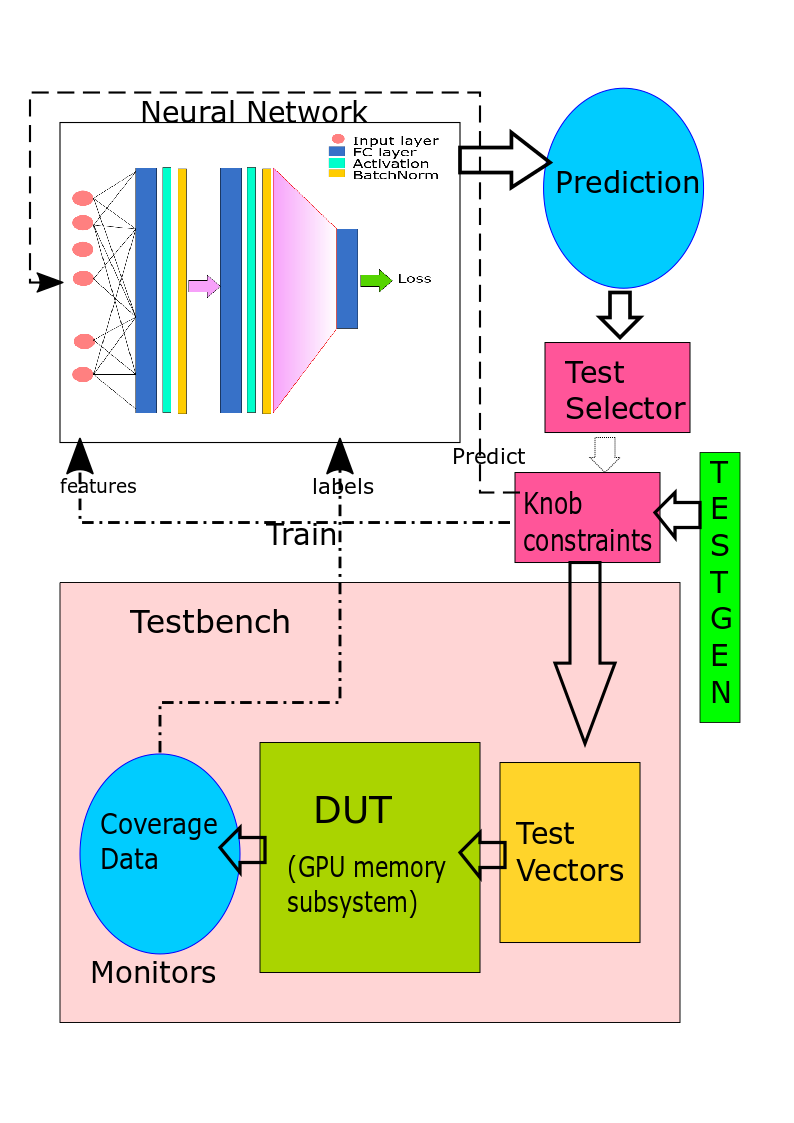
\includegraphics[trim={1cm 4.8cm 2cm 3.2cm},clip,scale=0.5]{Imagen1m.png}
    \caption{Arquitectura proceso de flujo}
    \end{figure}
    
    Esta columna está completamente destinada para los resultados y análisis de su investigación / trabajo. Puede agregar gráficos, tablas y los resultados que considere necesarios con sus respectivos análisis.
    
    \vspace{0.5cm}
    \begin{figure}
    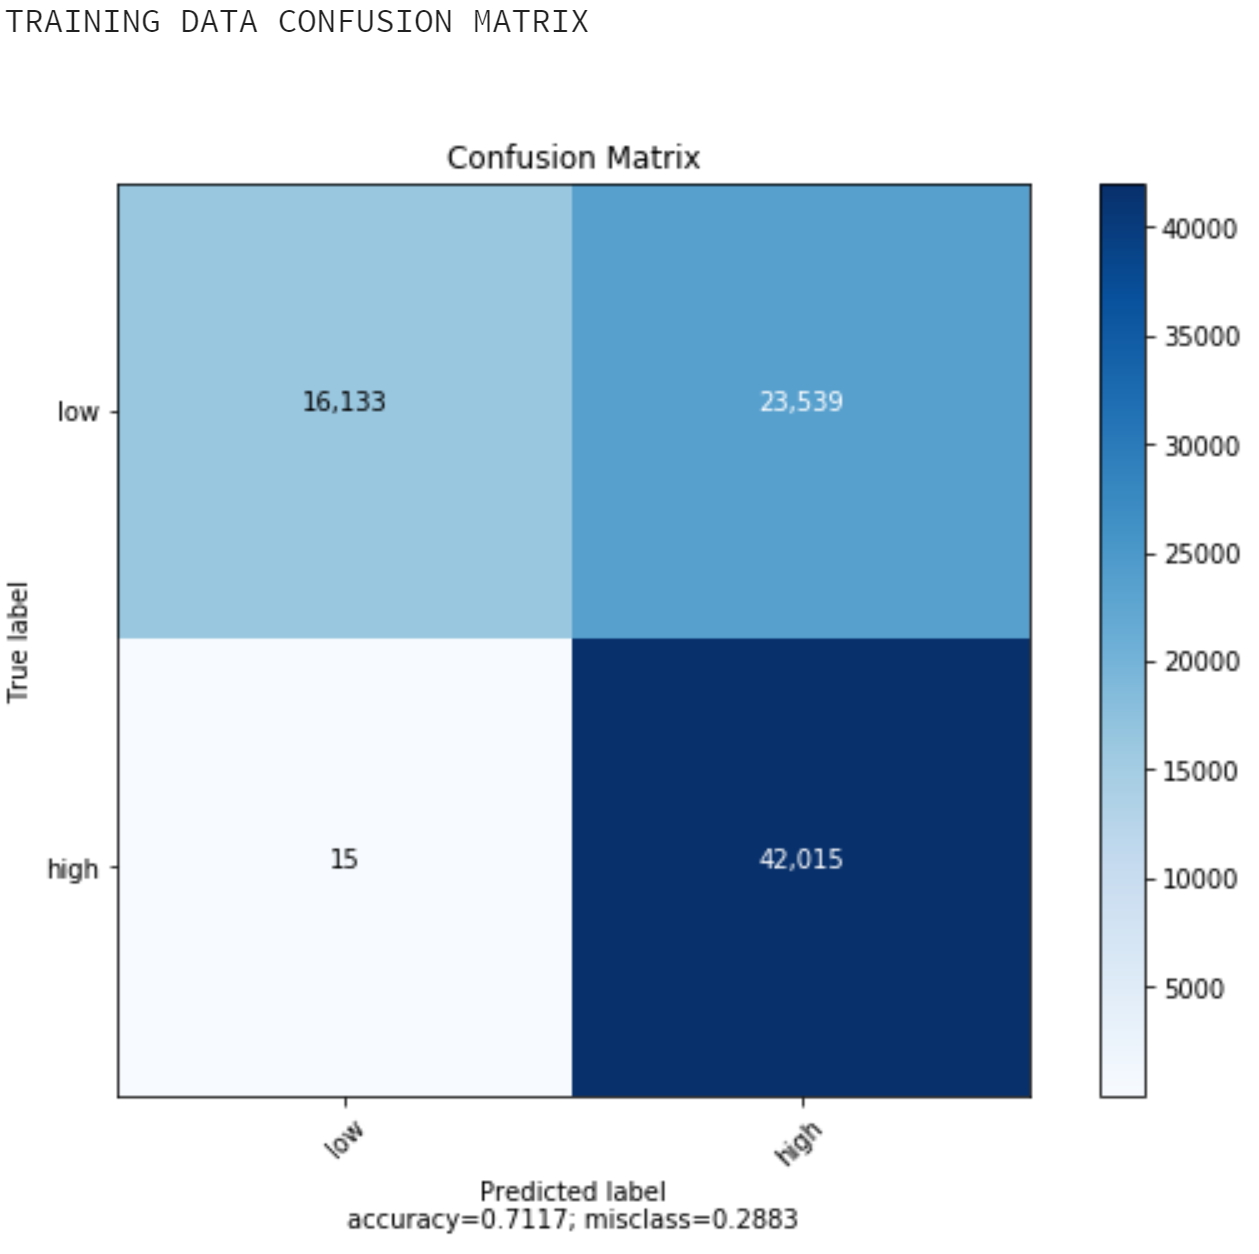
\includegraphics[trim={0 0 0 2cm},clip,scale=0.5]{Imagen2m.PNG}
    \caption{Comparación de cubierta verdadera y predicha}
    \end{figure}

    \begin{table}
        \centering
        \begin{tabular}{|l|c|c|c|}
            \hline
            \% tests & Coverage overlap & Selected CCS & Random CCS\\
            \hline
            2\%  &44.39\% &14.3 & 0.62 \\
            \hline
            5\% & 58.69\% &7.5 & 0.62 \\
            \hline
            10\%  &73.75\% &4.8 & 0.62 \\
            \hline
            \end{tabular}
        \caption{Mejora DL sobre muestreo aleatorio}
    \end{table}    
    

\end{block}


%----------------------------------------------------------------------------------------

\end{column} % Final de la primera columna

\begin{column}{\sepwid}\end{column} % Columna espaciadora vacía

%\begin{column}{\twocolwid} % Inicio de  La segunda columna 
\begin{column}{\onecolwid}




%----------------------------------------------------------------------------------------
%	CONCLUSIONES
%----------------------------------------------------------------------------------------

\begin{block}{Conclusiones}
Inserte aquí las principales conclusiones a las cuales llegó a partir de los resultados obtenidos y teniendo en cuenta los objetivos planteados en la sección correspondiente.

\vspace{0.5cm}
\begin{figure}
    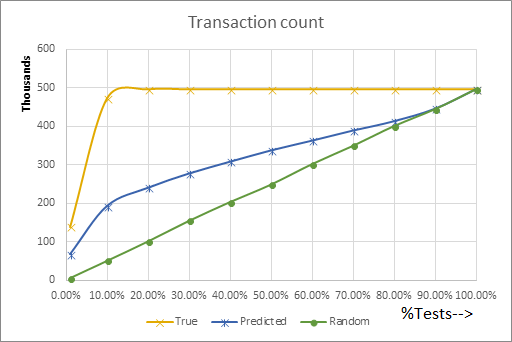
\includegraphics[width=0.8\textwidth]{Imagen3m.png}
    \caption{\ Comparación de recuento de transacciones de ruta única Verdadera/Predicha/Aleatoria}
\end{figure}

Inserte aquí las conclusiones secundarias a las cuales llegó a partir de los resultados obtenidos y teniendo en cuenta los objetivos planteados en la sección correspondiente.
\end{block}

%----------------------------------------------------------------------------------------
%	REFERENCIAS
%----------------------------------------------------------------------------------------


\begin{block}{Referencias}

\begin{itemize}
\item \href{https://www.researchgate.net/publication/220306081_Coverage-Directed_Test_Generation_Automated_by_Machine_Learning_-_A_Review}{Coverage directed testbench automation} 
\item \url{https://www.researchgate.net/publication/220306081_Coverage-Directed_Test_Generation_Automated_by_Machine_Learning_-_A_Review}{ Coverage directed testbench automation}
\item Automating Design Verification
\item \url{https://dvcon.org/sites/dvcon.org/files/files/2018/06_1.pdf}{ Deep predictive coverage collection}
\item \href{https://dvcon.org/sites/dvcon.org/files/files/2018/06_1.pdf}{Deep predictive coverage collection}
\end{itemize}
\end{block}





%----------------------------------------------------------------------------------------

%\begin{block}{RECOMENDACIONES}

%\end{block}

%----------------------------------------------------------------------------------------

%----------------------------------------------------------------------------------------
%	INFORMACIÓN ADICIONAL
%----------------------------------------------------------------------------------------


%----------------------------------------------------------------------------------------
%	AGRADECIMIENTOS
%-------------------------------------------------------------------


\end{column} % Final de la segunda columna

\begin{column}{\sepwid}\end{column} % Columna espaciadora vacía



\end{columns} % Final de todas las columnas del poster

\end{frame} % Final del entorno

\end{document} 
%% FIN DEL DOCUMENTO

